% app2.tex (will be Appendix B)

\Chapter{Bose Condensate and Thermal Cloud}
\label{sec:Bose}
%\label{app:tabfig}
We consider an interacting Bose condensate coupled with its thermal cloud confined in a special quasi-2D geometry , where its disk extends to infinity in both dimensions and there exists a parabolic lateral confinement which gives rise to interesting phenomena.

\section{Collective Modes of Confined Bose Condensate and Thermal Cloud for Harmonic Potential}
In this section we consider the collective modes of the condensate and thermal cloud for the harmonic potential. We call this geometry the ``Pancake" geometry.
\be
U(x,y,z) = \frac{m\omega_x^2x^2}{2}+\frac{m\omega_y^2y^2}{2}+\frac{m\omega_z^2z^2}{2}
\ee
for pancake geometry, $\omega_z\equiv\omega_\perp$, $\omega_y,\omega_z\rightarrow 0$. The condensate modes are provided by the solution of the following equations~\cite{Pethic}:
\be\label{BCcontinuity}
\frac{\partial \delta n}{\delta t} = -\bm{\nabla}\cdot\left(n_{eq}\bm{v}\right)
\ee
\be\label{BCEuler}
m\frac{\partial \bm{v}}{\partial t} = -\bm{\nabla}\left(\delta \tilde{\mu}\right) 
\ee
Under Thomas-Fermi approximation, the $\tilde{\mu}$ term reduces to a potential term and an interaction term:
\begin{align}
&\tilde{\mu} = U + nV_0 \\
\mathrm{or,} \ &\delta \tilde{\mu} = \delta nV_0
\end{align}

It should be noted that there is no entropy equation for the condensate as it does not carry entropy. The time-derivative of the continuity equation \eqref{BCcontinuity} yields:
\be
\frac{\partial^2 \delta n}{\partial t^2} = -\bm{\nabla}\cdot\left(n_{eq} \frac{\partial \bm{v}}{\partial t}\right) = \frac{V_0}{m}\bm{\nabla}\cdot\left(n_{eq}\bm{\nabla}\delta n\right)
\ee
\begin{figure}[h]
\begin{center}
%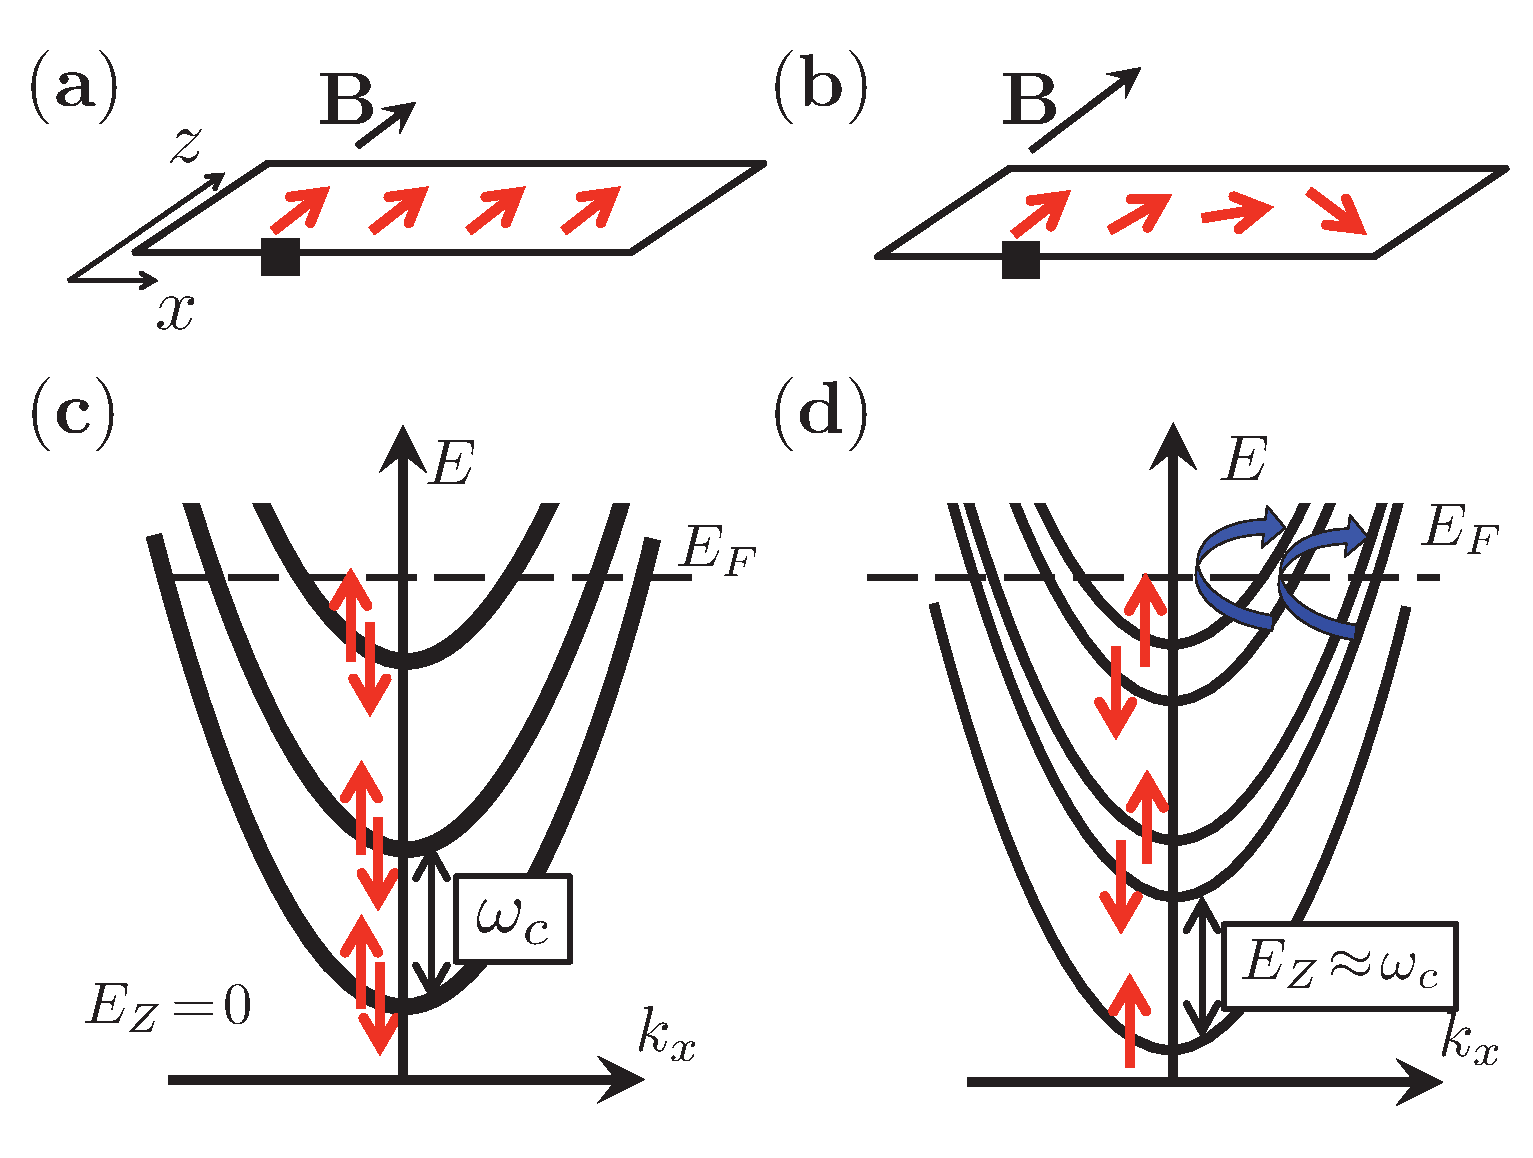
\includegraphics[width=1.0\columnwidth]{fig1.eps}
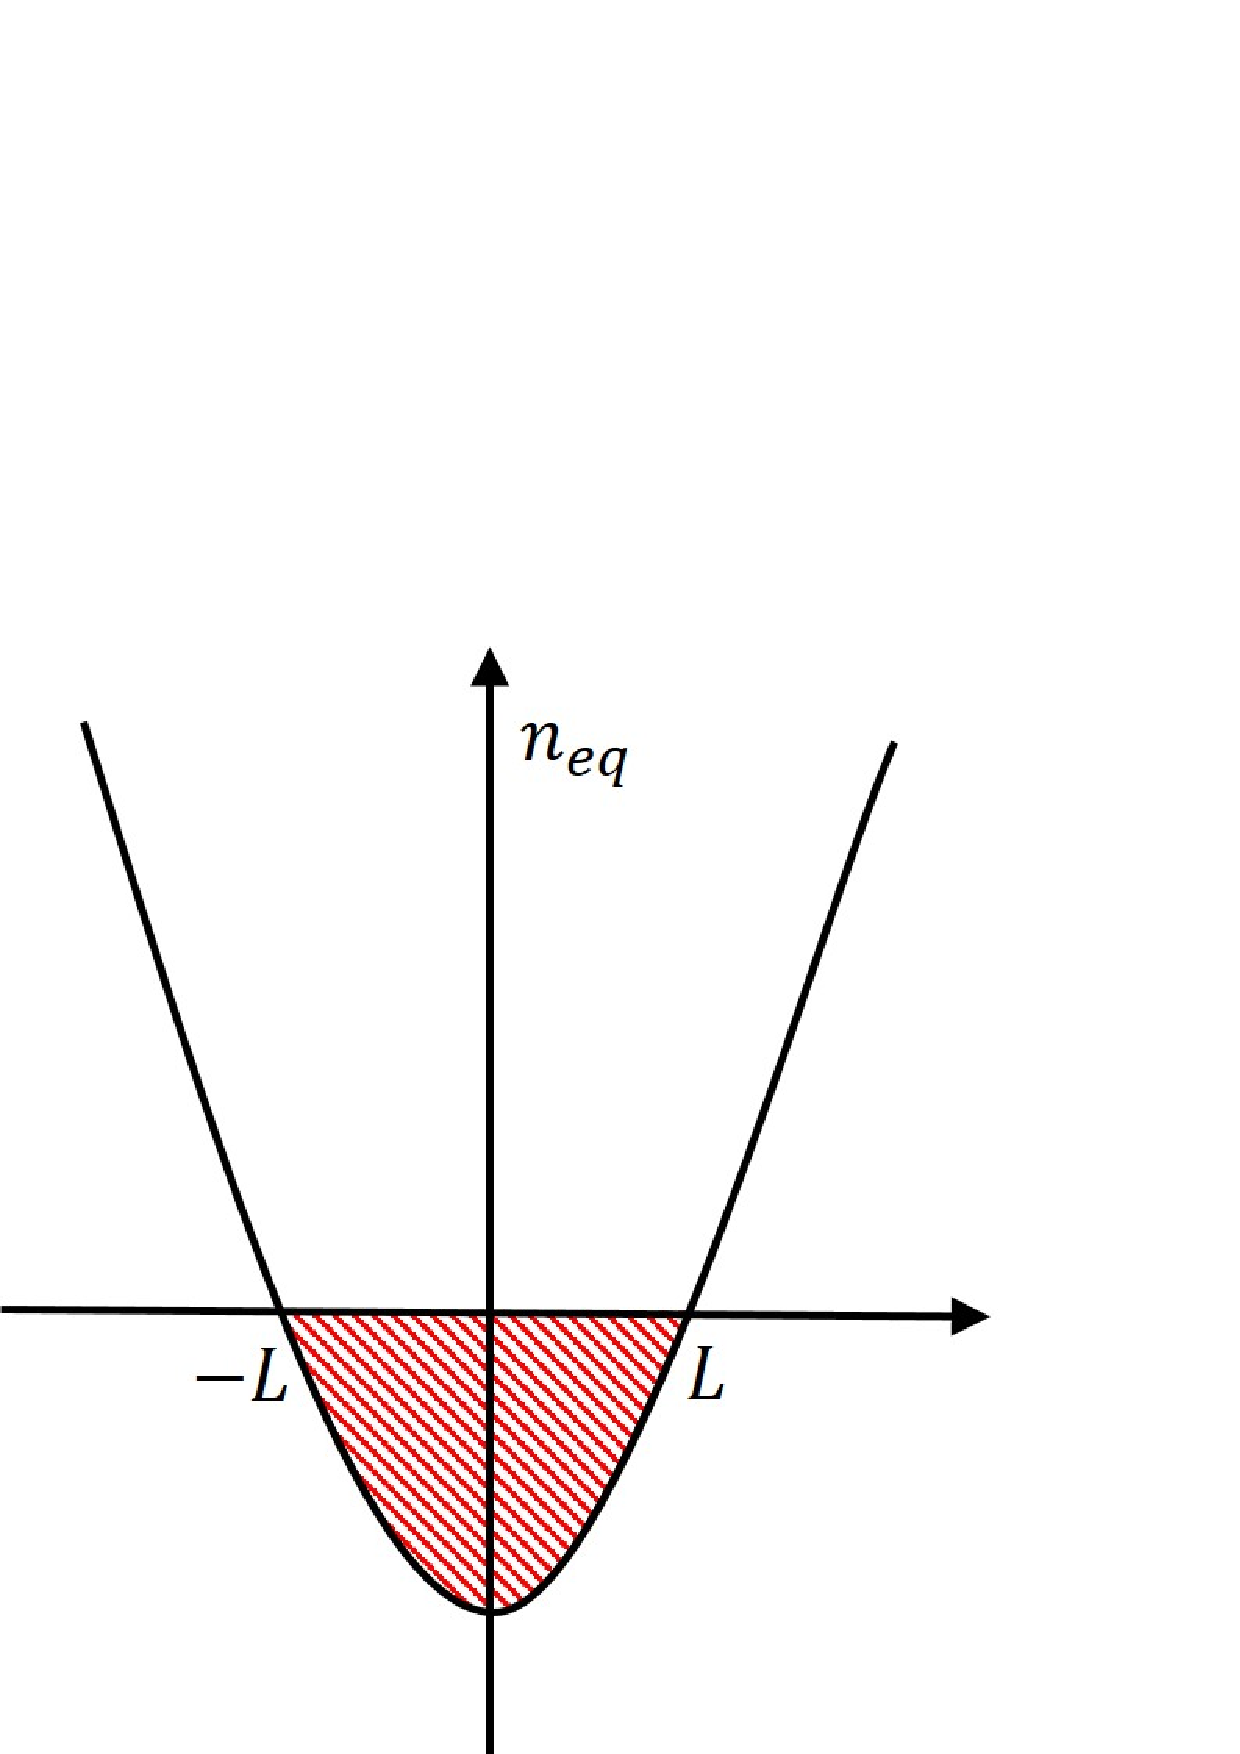
\includegraphics[height=0.5\columnwidth]{BC1.jpg}
\caption{The equilibrium density, $n_{eq}$ as a function of $\bm{z}$}
\label{fig:BC1}
\end{center}
\end{figure}

At equilibrium,
\be
\frac{kz^2}{2}+nV_0 \equiv \mathrm{const} = \frac{kL^2}{2}
\ee
where, L is the extent of the condensate, and
\be
n = n_0 \left(1-\left(\frac{z}{L}\right)^2\right)
\ee
where the parameter $n_0$ is given by
\be
n_0 = n(z=0) = \frac{kL^2}{2V_0}
\ee
These parameters set the conditions for the equilibrium density:
\be
m\frac{\partial^2 \delta n}{\partial t^2} = V_0 \bm{\nabla}\cdot \left(n_{eq} \bm{\nabla} \delta n \right)
\ee
or,
\be
\frac{m}{V_0} \frac{\partial^2 \delta n}{\partial t^2} = V_0 n_0 \partial_z \left(\left(1-\left(\frac{z}{L}\right)^2\right)\partial_z\delta n\right)
\ee
with the change of variable $z/L \equiv y$:
\be
\frac{L^2}{n_0} \frac{m}{V_0} \frac{\partial^2 \delta n}{\partial t^2} = \partial_y \left[\left(1-y^2\right)\partial_y \delta n\right]
\ee
But, we recognize that:
\be
\frac{L^2}{n_0} \frac{m}{V_0} = \frac{L^2m}{kL^2} \frac{2V_0}{V_0} = 2 \frac{m}{k} = \frac{2}{\omega_\perp^2}
\ee
Then we arrive at the following equation:
\be
\frac{\partial^2 \delta n}{\partial t^2} = \frac{\omega_\perp^2}{2} \partial_y \left[\left(1-y^2\right)\partial_y\delta n\right]
\ee
We  are particularly looking for solutions of the type $\delta n = \delta n_\omega e^{-i\omega t}$, which yields
\be
-\omega^2 \delta n_\omega = \frac{\omega_\perp^2}{2}\partial_y\left[\left(1-y^2\right)\partial_y\delta n\right]
\ee
We recognize this as the Legendre differential equation:
\be
\delta l^2 P_l = \frac{\omega_\perp^2}{2}\left[-l(l+1)P_l\right]
\ee
with
\be
\omega_l = \omega_\perp\sqrt{\frac{l(l+1)}{2}} \ , \ \delta n = P_l(y)e^{-i\omega t}
\ee
While $l=1$, $\delta n \propto n_0 y e^{-i\omega t}$. The time dependence of the velocity is given by:
\be
m\frac{\partial \bm{v}}{\partial t} = -V_0 \bm{\nabla}\delta n \Rightarrow -i\omega mv = -V_0n_0
\ee
So, the velocity $(\bm{v}(z)=\bm{v})$ is constant in space which is the Kohn mode of the condensate.

\section{Thermal Cloud in Pancake Geometry}
For the thermal cloud, we start by writing the continuity equation and the linearized Euler equation \cite{Pethic},
\bea
\frac{\partial \rho}{\partial t} + \bm{\nabla}\cdot(\rho \bm{v}) = 0 \\
\rho_{eq}\frac{\partial \bm{v}}{\partial t} = -\bm{\nabla}P + \rho\bm{f}
\eea
where, $\bm{f}$ is the force per unit mass: $\bm{f}=-\frac{1}{m}\bm{\nabla}V$, and at equilibrium, $\bm{\nabla}P_{eq}=\rho_{eq}\bm{f}$. Also, taking a time derivative of the previous equation:
\be\label{BCA*}
\rho_{eq} \frac{\partial^2 \bm{v}}{\partial t^2} = -\bm{\nabla} \left(\frac{\partial P}{\partial t}\right) + \frac{\partial \rho}{\partial t} \bm{f}
\ee
We specify the adiabatic conditions for ideal gas: $P/\rho^{5/3}=\textrm{const}$.
\subsection{The Case of a Monoatomic Classical Gas}
Here we will investigate the Kohn theorem for the pancake geometry in case of a classical monoatomic gas. We start by rewriting the adiabatic condition for ideal gas in the following form:
\be
\frac{dP}{P} + \frac{5}{3} \frac{d\mathcal{V}}{\mathcal{V}} = 0 
\ee
We know, for classical gas, $P\mathcal{V} = NkT$ and $E=\frac{3}{2} NkT$. With help of these relations, we find:
\be
dP = -\frac{NkT}{\mathcal{V}^2}d\mathcal{V} + \frac{NkdT}{\mathcal{V}} \ ; \ dE = \frac{3}{2}NkdT = -Pd\mathcal{V} (\mathrm{adiabatic \ compression})
\ee
and finally,
\be
dP=-\frac{P}{\mathcal{V}}d\mathcal{V}-\frac{2}{3}\frac{P}{\mathcal{V}}d\mathcal{V}=-\frac{5}{3}\frac{P}{\mathcal{V}}d\mathcal{V}
\ee
Now, we let $\bm{\xi}=\bm{v}dt$ be the displacement of the mass parcel of a fluid during time dt. As $P/\rho^{5/3}=\textrm{const}$, we have
\be
\frac{P(\bm{r}+\bm{\xi})}{\rho(\bm{r}+\bm{\xi})^{5/3}}=\frac{P_{eq}(\bm{r})}{\rho_{eq}^{5/3}(\bm{r})}
\ee
which yields,
\begin{align}
P(\bm{r})-P_{eq}(\bm{r}) &= \left(P_{eq}(\bm{r})-\bm{\xi}\frac{\partial P}{\partial \bm{r}}\right) \left[\frac{\rho_{eq}(\bm{r})+\delta\rho}{\rho_{eq}(\bm{r})-\bm{\xi}.\bm{\nabla}\rho_{eq}}\right]^{5/3}-P_{eq} \\
&= -\bm{\xi}\cdot\bm{\nabla}P_{eq}+\frac{5}{3}\frac{P_{eq}}{\rho_{eq}}\left(\delta \rho+\bm{\xi}\cdot\bm{\nabla}\rho_{eq}\right)
\end{align}
With $\bm{v}=\dot{\bm{\xi}}$:
\be\label{BCA1}
\frac{\partial P}{\partial t} = \frac{5}{3} \frac{P_eq}{\rho_eq}\left(\partial \delta \rho{\partial t} + \bm{v}\cdot\bm{\nabla}\rho_{eq}\right) - \bm{v}\cdot\bm{\nabla} P_{eq}
\ee
The continuity equation gives:
\be
\frac{\partial \delta \rho}{\partial t} + \bm{v}\cdot\bm{\nabla}\rho_{eq}+\rho_{eq}\bm{\nabla}\cdot\bm{v}=0
\ee
Then equation \eqref{BCA1} becomes:
\begin{align}
\frac{\partial P}{\partial t} &= -\frac{5}{3}P_{eq}\bm{\nabla}\cdot\bm{v}-\bm{v}\cdot\bm{\nabla}P_{eq} \\
&= -\frac{5}{3}P_{eq}\bm{\nabla}\cdot\bm{v}-\rho_{eq}\bm{f}\cdot\bm{v}
\end{align}
Thus,
\be\label{BCA**}
\frac{\partial P}{\partial t} = -\frac{5}{3}P_{eq}\bm{\nabla}\cdot\bm{v}-\rho_{eq}\bm{f}\cdot\bm{v}
\ee
At equilibrium, $P_{eq}=P_{eq}(\rho_{eq}.T)$.
\be
\bm{\nabla}P_{eq}=\frac{\partial P_{eq}}{\partial \rho_{eq}}\bm{\nabla}\rho_{eq}=\rho_{eq}\bm{f}
\ee
which means $\bm{\nabla}\rho_{eq}\parallel\bm{f}$
\be
(\bm{f}\cdot\bm{v})\bm{\nabla}\rho_{eq}=\bm{f}(\bm{v}\cdot\bm{\nabla})\rho_{eq}
\ee
Using equations \eqref{BCA*} and \eqref{BCA**}, we get:
\be
\frac{\partial^2 \bm{v}}{\partial t^2} = \frac{5}{3}\frac{P_{eq}}{\rho_{eq}}\bm{\nabla}(\bm{\nabla}\cdot\bm{v})+\bm{\nabla}(\bm{f}\cdot\bm{v})+\frac{2}{3}(\bm{\nabla}\cdot\bm{v})\bm{f}
\ee

For classical Gas, $\frac{p_{eq}}{\rho_{eq}}=\frac{kT}{m}$. Also, $\bm{v}(t)=\bm{v}e^{-i\omega t}$, $\bm{v}=(0,0,v)$, and for pancake geometry, $\bm{f}=-\omega_\perp^2z\hat{\bm{z}}$. Applying these conditions,
\be
-\omega^2v = \frac{5}{3} \frac{kT}{m} \partial_z^2v - \partial_z(\omega_\perp^2zv) - \frac{2}{3}\omega_\perp^2z\partial_zv
\ee
With the change of variables $z=y\sqrt{2kT/m\omega_\perp^2}$,
\be
\frac{6}{5\omega_\perp^2}(-\omega^2+\omega_\perp^2)v = \partial_y^2v - 2y\partial_yv
\ee
Which has the solution in the form of Hermite polynomial $v_n(y)-v_0H_n(y)$. $H_n(y)$ satisfies $y''-2xy'+2ny=0$. Thus, we have
\bea
\frac{6}{5\omega_\perp^2}(-\omega^2+\omega_\perp^2)H=-2nH_n \\
\omega=\omega_\perp\left(\frac{3+5n}{3}\right)^{1/2}
\eea
For $n=0$, $v_{n=0}=H_0(y)\equiv const$, $\omega=\omega_\perp\left(\frac{3+5\times 0}{3}\right)^{1/2}=\omega_\perp$. This is the Kohn theorem for the thermal cloud.
%\newpage

%%%%%%%%%%%%%%%%%%%%%%%%%%%%%%%%%%%%%%%%%%%%%
\section{The Coupled System}
%\label{app:tabfig:tables}
Here, we wish to investigate the behavior of the Bose condensate coupled with its thermal cloud confined inside the pancake geometry. To achieve this, first we need to write the complete sets of coupled equations for each of the two. Firstly, the complete Equations for Condensate are \cite{zaremba1998},
\bea 
\frac{\partial n_c}{\partial t} = - \bm{\nabla}\cdot \left(n_c \bm{v}_c\right) \\
m\left( \frac{\partial\bm{v}_c}{\partial t} + \frac{1}{2} \bm{\nabla}v^2_c \right) = - \bm{\nabla}\phi 
\eea
where,
\bea 
\bm{v}_c(\bm{r},t) \equiv \frac{\hbar}{m} \bm{\nabla} \theta (\bm{r},t) \\
\phi (\bm{r},t) \equiv \frac{1}{|\Phi(\bm{r},t)|} \hat{H}(\bm{r},t) |\Phi(\bm{r},t)| \\
\hat{H}(\bm{r},t) = - \frac{\hbar^2 \bm{\nabla}^2}{2m} + U (\bm{r}) + 2g\tilde{n}(\bm{r},t) + gn_c(\bm{r},t) \\
\Phi(\bm{r},t)=|\Phi(\bm{r},t)|e^{i\theta(\bm{r},t)} \\
n_c(\bm{r},t) = |\Phi(\bm({r},t)|^2 \\
g = 4\pi a \hbar^2/m
\eea

And now, the complete equations for thermal cloud are,
\bea
\frac{\partial\tilde{n}}{\partial t} + \bm{\nabla}\cdot(\tilde{n}\bm{v}_n) = 0 \\
m\tilde{n} \left( \frac{\partial\bm{v}_n}{\partial t} + (\bm{v}_n\cdot\bm{\nabla})\bm{v}_n \right) = -\bm{\nabla}\tilde{P} - \tilde{n}\bm{\nabla}U \\
\frac{\partial\tilde{\epsilon}}{\partial t} + \frac{5}{3} \ \bm{\nabla} \cdot (\tilde{\epsilon}\bm{v}_n) = \bm{v}_n \cdot \bm{\nabla}\tilde{P}
\eea

where,
\be \tilde{n}(\bm{r},t) \equiv \int \frac{d^3p}{h^3} f_0(\bm{r},\bm{p},t) = \frac{1}{\Lambda^3} g^{3/2}(z(\bm{r},t)) \ee
with,
\bea
z(\bm{r},t) \equiv e^{\beta(\bm{r},t)\left[\mu(\bm{r},t)-U(\bm{r},t)\right]} \\
\Lambda(\bm{r},t) = 2\pi\hbar^2/mk_BT(\bm{r},t)^{1/2} \\
f_0(\bm{r},\bm{p},t) = \left[exp\left[\beta\{\frac{1}{2m}\left[\bm{p}-m\bm{v}_n\right]^2+U-\mu\}\right]-1\right]^{-1} 
\eea

$\tilde{\epsilon}$ is the non-convective part of kinetic energy density
\bea
\tilde{P} = \frac{2}{3}\tilde{\epsilon} \\
\bm{\nabla}\tilde{P}=-\tilde{n}_0\bm{\nabla}U_0
\eea
where,
\be U_0 = U + 2g\tilde{n}_0 + 2gn_{c0} \ee
The eigenvalue equation for the Hamiltonian operator is,
\be \label{BCBA}
H\Phi=\left(U+2g\tilde{n}+gn_c\right)\Phi
\ee
We define $\phi$ as,
\be
\phi \equiv \frac{1}{|\Phi|} H|\Phi| = U + 2g\tilde{n}+gn_c
\ee
or,
\be
\delta \phi = 2g\delta\tilde{n}+g\delta n_c
\ee

Next, we linearize both of the system of equations. For the condensate, we have
\be\label{BCB1a}
\frac{\partial\delta n_c}{\partial t} = -\bm{\nabla} \cdot (n_{c0}\delta\bm{v}_c)
\ee
\be\label{BCB1b}
m \frac{\partial\delta\bm{v}_c}{\partial t} = -\bm{\nabla}\delta\phi 
\ee

and for thermal cloud,
\be\label{BCB2a}
\frac{\partial\delta\tilde{n}}{\partial t} = -\bm{\nabla}.(\tilde{n}_0\delta\bm{v}_n)
\ee
\be\label{BCB2b}
m\tilde{n}_0\frac{\partial\delta\bm{v}_n}{\delta t} = -\bm{\nabla}\delta\tilde{P}-\delta\tilde{n}\bm{\nabla}U_0-2g\tilde{n}_0\bm{\nabla}(\delta\tilde{n}+\delta n_c)
\ee
\be\label{BCB2c}
\frac{\partial \delta\tilde{P}}{\partial t} = - \frac{5}{3} \ \bm{\nabla} \cdot (\tilde{P}_0\delta\bm{v}_n)+\frac{2}{3} \ \delta\bm{v}_n \cdot \bm{\nabla}\tilde{P}_0
\ee

\subsection{Verification of Kohn Mode}
To verify the Kohn theorem, we consider the small displacement of kind
\be\label{BCB3}
\bm{\eta}(t) = \bm{\eta}_0 cos\omega_it
\ee
The confinement potential is of the shape
\be\label{BCB4}
U = \frac{1}{2} \ m(\omega_x^2x^2+\omega_y^2y^2+\omega_z^2z^2)
\ee
Therefore,
\be\label{BCB5}
\delta\tilde{n}=-\bm{\nabla}\tilde{n}_0 \cdot \bm{\eta}(t) \ \ \ \delta n_c = -\bm{\nabla}n_{c0} \cdot \bm{\eta}(t)
\ee
and,
\be\label{BCB6}
\delta\bm{v}_c = \delta\bm{v}_n = \dot{\bm{\eta}}(t)
\ee
It is important to note that the above equation \eqref{BCB6} is spatially independent. Now, there are three possible choices for $\bm{\eta}$, namely, $\eta \hat{\bm{x}}$, $\eta \hat{\bm{y}}$ and $\eta \hat{\bm{z}}$. We choose to take $\bm{\eta}=\eta \hat{\bm{z}}$ for definiteness.

First observe that equation \eqref{BCB1a} is valid. With use of \eqref{BCB5}, we can rewrite it as:
\be 
 \frac{\partial}{\partial t} \left(-\bm{\nabla}n_{c0} \cdot \bm{\eta} \right) = -\bm{\nabla} \cdot \left(n_{c0} \dot{\bm{\eta}}\right) \ee
which is valid because $n_{c0}$ is independent of $t$ and $\bm{\eta}$ is independent of space.

Now, equation \eqref{BCB1b}:
\be m \frac{\partial\delta\bm{v}_c}{\partial t} = -\bm{\nabla}\delta\phi \ee
from \eqref{BCBA} and \eqref{BCB6}:
\be\label{BCB7}
m \frac{\partial}{\partial t} \dot{\bm{\eta}}(t) = -\bm{\nabla}(2g\delta\tilde{n}+g\delta n_c)
\ee
using \eqref{BCB5}:
\bea
m \frac{\partial}{\partial t} \dot{\bm{\eta}}=-g\bm{\nabla} \cdot (-2\bm{\nabla}\tilde{n}_0 \cdot \bm{\eta}(t)-\bm{\nabla}n_{c0} \cdot \bm{\eta}(t)) \\
m \frac{\partial}{\partial t} \dot{\bm{\eta}} = g\bm{\nabla}(\bm{\nabla}(2\tilde{n}_0+n_{c0}) \cdot \bm{\eta})
\eea
with $\bm{\eta}=\eta \hat{\bm{z}}$,
\be
-m\omega_z^2\cos{(\omega_zt)}\eta_0\hat{\bm{z}}=g\bm{\nabla}\cdot(\partial_z(2\tilde{n}_0+n_{c0})\eta_0\cos{(\omega_zt)})
\ee
or,
\be
\partial_z^2(g(2\tilde{n}_0+n_{c0})+\frac{1}{2} \ m\omega_z^2z^2)=0
\ee
which is correct because $(\frac{1}{2} \ m\omega_z^2z^2+2g\tilde{n}_0+gn_{c0})$ is constant in $(x,y,z)$. \\
Now, we will verify equations \eqref{BCB1a} through \eqref{BCB2c}. First, from equation \eqref{BCB2a},
\bea
\frac{\partial\delta\tilde{n}}{\partial t} = -\bm{\nabla}\cdot(\tilde{n}_0\delta\tilde{v}_n) \\
\mathrm{or,} \frac{\partial}{\partial t}(-\bm{\nabla}\tilde{n}_0\cdot\bm{\eta})=-\bm{\nabla}\cdot(\tilde{n}_0\frac{\partial}{\partial t}\bm{\eta})
\eea
which is evidently a valid relation. Now, from equation \eqref{BCB2c}, we have
\begin{align}
\frac{\partial\delta\tilde{P}}{\partial t} &= - \frac{5}{3} \ \bm{\nabla}.(\tilde{P}_0\delta\bm{v}_n)+\frac{2}{3} \ \delta\bm{v}_n\cdot\bm{\nabla}\tilde{p}_0 \\
&= -\frac{5}{3} \ (\bm{\nabla}\tilde{P}_0)\cdot\dot{\bm{\eta}}+\frac{2}{3} \ (\bm{\nabla}\tilde{P}_0)\cdot\dot{\bm{\eta}} \\
&= - (\bm{\nabla}\tilde{P}_0)\cdot\dot{\bm{\eta}}
\end{align}

which gives us,
\be\label{BCB8}
\delta\tilde{P} = -(\bm{\nabla}\tilde{P}_0)\cdot\bm{\eta}
\ee

Equation \eqref{BCB2b}, with help of \eqref{BCB8} can be rewritten as
\be
m\tilde{n}_0 \frac{\partial}{\partial t}\dot{\bm{\eta}} = -\bm{\nabla}\left[(-\bm{\nabla}\tilde{P}_0)\cdot\bm{\eta}\right] - \left[(-\bm{\nabla}\tilde{n}_0)\cdot\bm{\eta}\right]\bm{\nabla}U_0-2g\tilde{n}_0(\bm{\nabla}\delta\tilde{n}+\bm{\nabla}\delta n_c)
\ee
using equation \eqref{BCB7} with $\bm{\eta}=\eta\hat{\bm{z}}$ (considering z-components only),
\be
-\tilde{n}_0\partial_z(2g\delta\tilde{n}+g\delta n_c) = (\partial_z^2\tilde{P}_0)\eta+(\partial_z\tilde{n}_0)(\partial_zU_0)\eta-2g\tilde{n}_0\partial_z(\delta\tilde{n}+\delta n_c)
\ee
or,
\be\label{BCB9}
\partial_z^2\tilde{P}_0\eta+(\partial_z\tilde{n}_0)(\partial_zU_0)\eta-g\tilde{n}_0\partial_z\delta n_c =0
\ee
but, we know, $\bm{\nabla}\tilde{P}_0=-\tilde{n}_0\bm{\nabla}U_0$. Then \eqref{BCB9} reduces to
\be
-\partial_z^2\left[U+2g\tilde{n}_0+gn_{c0}\right]=0
\ee
which is correct because $U+2g\tilde{n}_0+gn_{c0}$ is constant in $z$.
%AI
This proves that the collective oscillations in our confined condensate-thermal cloud system are protected from interactions and the Kohn theorem holds for such systems.

\section{Anharmonicity in the Condensate}
%AI
Here we will investigate the effects of potential anharmonicity in the condensate. We start with the linearized equations as before:
\be\label{BCC1}
\frac{m}{U_0} \frac{\partial^2\delta n}{\partial t^2} = U_0 \bm{\nabla} (n_{eq}\bm{\nabla}\delta n)
\ee
Now we introduce a small non-parabolicity controlled by the parameter $\varepsilon$:
\bea\label{BCC2}
n_{eq} = \frac{1}{U_0} \frac{k(L^2-z^2)}{2} + \varepsilon\frac{(z^4-L^4)}{4} \\
= n_0 \left(1-\left(\frac{z}{L}\right)^2\right) + n_1\left(\left(\frac{z}{L}\right)^4-1\right)
\eea

where, $n_0 \equiv \frac{kL^2}{2U_0}$ \& $n_1 \equiv \frac{\varepsilon L^4}{4}$ \\
from equation \eqref{BCC1}:
\be
\frac{\partial^2\delta n}{\partial t^2} = \frac{U_0}{m} \frac{\partial}{\partial z} \left[\left[n_0\left(1-\left(\frac{z}{L}\right)^2\right) + n_1\left(\left(\frac{z}{L}\right)^4-1\right)\right]\frac{\partial}{\partial z}\delta n\right]
\ee
now, we consider $\delta n \propto e^{-i\omega t}$ and a change of variable $\frac{x}{L} = y$
\be
-\omega^2\delta n = \frac{n_0U_0}{mL^2} \frac{\partial}{\partial y} \left[\left[\left(1-y^2\right)+\frac{n_1}{n_0}\left(y^4-1\right)\right]\frac{\partial}{\partial y} \delta n\right]
\ee
with $\frac{\omega_\perp^2}{2}$:
\be
-\omega^2\delta n = \frac{\omega_\perp^2}{2} \frac{\partial}{\partial y} \left[\left(1-y^2\right)\frac{\partial}{\partial y}\delta n\right] + \frac{\omega_\perp^2}{2} \frac{n_1}{n_0} \frac{\partial}{\partial y} \left[\left(y^4-1\right)\frac{\partial}{\partial y}\delta n\right]
\ee
with $\lambda\equiv\omega^2$, we arrive at the eigenvalue equation, which is just the Legendre differential equation:
\bea
\lambda\delta n = -\frac{\omega_\perp^2}{2} \ \frac{\partial}{\partial y}\left[\left(1-y^2\right)\frac{\partial}{\partial y}\right]\partial n \\
\lambda = l(l+1), l=0,1,2,3,... \\
\delta n_l(y)=P_l(y)\sqrt{\frac{2l+1}{2}}
\eea
\\
so far we have:
\be
\lambda\delta n = H_0 + H_1
\ee
where, $H_0\equiv-\frac{\omega_\perp^2}{2} \frac{\partial}{\partial y} \left[\left(1-y^2\right)\frac{\partial}{\partial y}\delta n\right]$ and $H_1\equiv-\frac{\omega_\perp^2}{2}\frac{n_1}{n_0}\frac{\partial}{\partial y}\left[\left(y^4-1\right)\frac{\partial}{\partial y}\delta n\right]$ \\
with, $\lambda_l^0 = l(l+1)$ and $\delta n_l^0 = \sqrt{\frac{2l+1}{2}} \ P_l(y)\equiv f_l^0$. Now, we want to find the first order correction to the eigenvalue: $\lambda_l^1$.
\bea
\lambda_l^1=\left<f_l^0|H_1|f_l^0\right> \\
= - \left(\frac{2l+1}{2}\right) \frac{\omega_\perp^2}{2} \frac{n_1}{n_0} \int_{-1}^{1}P_l(y)\frac{\partial}{\partial y}\left[\left(y^4-1\right)\frac{\partial}{\partial y}P_l(y)\right]dy \\
\Rightarrow \lambda_1^1 = -\left(\frac{\omega_\perp^2}{2} \frac{n_1}{n_0}\right)\left(\frac{12}{5}\right)
\eea

\section{Anharmonicity in the Thermal Cloud}
We start with the usual equations:
\be\label{BCD1}
\frac{6}{5} \frac{1}{\omega_\perp^2} (-\omega^2+\omega_\perp^2)v=\partial_y^2v-2y\partial_yv
\ee
\be\label{BCD2}
\frac{\partial^2\bm{v}}{\partial t^2} = \frac{5}{3} \frac{P_{eq}}{\rho_{eq}}\bm{\nabla}(\bm{\nabla}\cdot\bm{v})+\bm{\nabla}(\bm{f}\cdot\bm{v})+\frac{2}{3}(\bm{\nabla}\cdot\bm{v})\bm{f}
\ee
For classical gas, $\frac{P_{eq}}{\rho_{eq}} = \frac{kT}{m}$. We also consider $v\propto e^{-i\omega t}\bm{x}$. Under These considerations, $\bm{f}$ takes the form:
\be
\begin{split}
\bm{f} & = -\bm{\nabla}U = -\frac{\partial}{\partial z} \left[\frac{1}{2} \omega_\perp^2 z^2 + \frac{\varepsilon}{4m}\left(z^4-L^4\right)\right]\hat{\bm{z}} \\
& = \left(-\omega_\perp^2z - \frac{\varepsilon}{m}z^3\right)\bm{z} \\
& \equiv (f_0 + f_1)\bm{z}
\end{split}
\ee
Then \eqref{BCD2} becomes:
\be\label{BCD3}
-\omega^2v=\frac{5}{3} \frac{kT}{m} \frac{\partial^2v}{\partial z^2}-\frac{\partial}{\partial z} \left(\omega_\perp^2zv+\frac{\varepsilon}{m}z^3\frac{\partial v_z}{\partial z}\right)
\ee
or,
\be
\left(-\omega^2+\omega_\perp^2\right)v=\frac{5}{3}\frac{kT}{m}\frac{\partial^2v}{\partial z^2}-\frac{5}{3}\omega_\perp^2z\frac{\partial v}{\partial z}-\frac{3\varepsilon}{m}z^2v-\frac{5}{3}\frac{\varepsilon}{m}z^3\frac{\partial v}{\partial z}
\ee
Performing a change of variable: $x\equiv y\sqrt{2kT/m\omega_\perp^2}$ and substituting $\eta\equiv\left(\frac{m\omega_\perp^2}{2kT}\right)^\frac{1}{2}$, we arrive at the following equation:
\be
\frac{6}{5} \left(\frac{-\omega^2+\omega_\perp^2}{\omega_\perp^2}\right)v=\frac{\partial^2 v}{\partial y^2} - 2y\frac{\partial v}{\partial y} - \frac{18\varepsilon}{5\eta^2m}y^2v-\frac{2\varepsilon}{\eta^2m}y^3\frac{\partial v}{\partial y}
\ee
we define:
\begin{align}
\lambda &\equiv \frac{6}{5} \left(\frac{-\omega^2+\omega_\perp^2}{\omega_\perp^2}\right) \\
H_0 &\equiv \frac{\partial^2 v}{\partial y^2} - 2y\frac{\partial v}{\partial y} \\
H_1 &\equiv - \frac{18\varepsilon}{5\eta^2m}y^2v-\frac{2\varepsilon}{\eta^2m}y^3\frac{\partial v}{\partial y}
\end{align}


Then the equation $H_0v=\lambda v$ is the Hermite polynomial equation. Thus,
\begin{align}
&\frac{6}{5}\left(\frac{-{\omega_n^0}^2+\omega_\perp^2}{\omega_\perp^2}\right) = -2n \\
\Rightarrow \ \ &{\omega_n^0}^2 = \left(1+\frac{5}{3}n\right)\omega_\perp^2 \\
&\lambda_n^0 \equiv \frac{6}{5}\left(\frac{-{\omega_n^0}^2+\omega_\perp^2}{\omega_\perp^2}\right)
\end{align}

The first-order corrections to the eigenvalues are given by:
\begin{align}
\lambda_n^1 &= \left(\frac{1}{\sqrt{\pi}2^nn!}\right) \int_{-\infty}^\infty H_n\hat{H}_1H_ne^{-y^2}dy \\
\lambda_0^1 &= -\frac{9\varepsilon}{5\eta^2m}
\end{align}
%\section{Some Figures}
%\label{app:tabfig:figures}

